
\documentclass[UTF8]{ctexart}
%================================ PREAMBLE ==================================

%--------- Packages -----------
\usepackage{fullpage}
\usepackage{amssymb}
\usepackage{amsmath}
\usepackage{amsthm}
\usepackage{latexsym}
\usepackage{graphicx}
\usepackage{wrapfig}
\usepackage{color}
%\usepackage{algorithm,algorithmic}
\usepackage{url}
\usepackage[round]{natbib}
\usepackage[scheme=plain]{ctex}%大写变为小写
\usepackage{lipsum}
\usepackage[colorlinks=true,citecolor=blue]{hyperref}
 
%----------Spacing-------------
%\setlength{\oddsidemargin}{0.25 in}
%\setlength{\evensidemargin}{-0.25 in}
\setlength{\topmargin}{-0.6 in}
%\setlength{\textwidth}{6.5 in}
%\setlength{\textheight}{9.4 in}
\setlength{\headsep}{0.75 in}
\setlength{\parindent}{0 in}
\setlength{\parskip}{0.1 in}

%----------Header--------------
\title{上海市二手房房价影响因素分析研究报告大纲}


\begin{document}
\maketitle%输出标题
\newpage%另起一页
\tableofcontents%命令输出论文目录
\newpage

\section{研究背景} 

\subsection{上海市房地产市场发展现状与行业特征} 

房地产行业是我国国民经济的支柱产业之一，而上海作为我国长三角核心超大城市、全国
房地产市场的标杆城市，其房地产市场运行规律、价格波动特征对全国楼市具有极强的示
范与引导作用。近年来，随着我国房地产市场从高速增量开发转向存量提质发展，上海新
房市场供给严格受限、二手房市场已成为城市住房流通、交易定价的核心主场，二手房房
价走势、空间分布规律，也成为反映上海房地产市场健康程度、城市资源配置效率的核心
指标。

从市场结构来看，上海二手房市场呈现高度微观分化、空间非均衡分布的典型特征。城市
内环、中环、外环间房价梯度差异显著，优质学区、轨道交通、商业医疗配套集中的中心
城区小区房价显著高于远郊区域；同时同一行政区内，相邻小区之间也存在明显的房价联
动、互相影响的特征，传统独立同分布的经典计量模型，已经无法解释上海二手房房价的
微观空间聚集、空间溢出规律。从行业发展特征来看，当前上海楼市已告别普涨周期，政
策端坚持 “房住不炒” 定位、落实稳地价稳房价稳预期目标，市场定价逻辑从单纯板块溢
价，逐步转向小区自身品质、周边公共服务配套、区位通达性等微观因素的综合定价，地
铁通勤、优质教育、生态环境、物业服务等微观配套因素，对二手房房价的影响持续深化。

与此同时，上海城市内部公共服务资源空间分布不均、轨道交通网络持续加密，进一步加
剧了二手房房价的空间关联性：优质配套资源不仅会抬升本小区房价，还会通过空间溢出
效应带动周边相邻小区房价同步上涨，形成高房价聚集片区；而配套薄弱区域则持续形成
低房价聚集片区。这种微观空间单元（小区层面）的房价空间联动性，是上海房地产市场
现阶段最核心的行业特征，也为本研究从微观空间计量视角，开展二手房房价影响因素实
证分析提供了现实基础。

\subsection{二手房房价影响因素的研究意义} 

理论层面，现有二手房房价影响因素研究多基于传统截面回归模型，默认不同小区房价相
互独立，忽略了城市内部微观空间单元的空间相关性与空间溢出效应，无法精准识别配套
因素对房价的直接影响与跨小区溢出效应。本文以上海微观小区二手房为研究对象，引入
空间计量模型、构建地理空间权重矩阵，通过全局 Moran's I 指数检验房价空间聚集特
征，运用空间杜宾模型（SDM）量化各影响因素的直接效应与空间溢出间接效应，弥补传
统计量方法的理论缺陷，完善超大城市二手房微观定价、空间经济学相关研究体系。

现实实践层面，本次研究具备多重应用价值。对购房者而言，可清晰识别地铁、学区、房
龄、物业等核心因素对房价的影响幅度与空间辐射范围，为理性置业选址、房价估值判断
提供科学参考；对房产中介、房企机构而言，能够掌握二手房微观定价逻辑与相邻板块溢
出规律，优化房源估值定价、市场研判策略；对城市规划、住建管理部门而言，可明确公
共服务配套的空间溢价效应，为上海学区均衡化、轨道交通规划、城市公共资源优化配置
、房地产市场平稳调控提供实证数据支撑，助力上海房地产市场健康可持续发展。

\section{数据来源与数据预处理}

\subsection{数据来源与整体说明} 

本研究的核心数据集来源于 Kaggle 平台公开的上海二手房数据集，该数据集全面覆盖了
上海市范围内的二手房房源信息，共包含 175,128 条有效记录，无缺失值，本数据集涵盖房源基
本属性、小区环境特征、区位配套条件、交易与产权信息等多个维度，能够较为完整反映上海二手房
市场的价格形成机制、房源分布特征及供需匹配情况。数据采集范围覆盖上海市各行政区及街道，
样本量大且分布均衡，具有较强的代表性，可有效满足区域差异分析、价格影响因素挖掘等研究目标。

为实现二手房市场的空间分布特征分析、区位价值评估等空间相关研究，需补充上海市小区经纬度
空间数据。由于核心数据集已包含 “小区名称”“区”“街道” 等精准地址信息，采用地理编码转换
方式获取经纬度坐标：通过调用高德地图 Web 服务 API，将 “上海市 + 区 + 街道 + 小区名称” 
的完整地址组合转换为 WGS84 坐标系下的经度、纬度数据，构建空间矩阵。


\subsection{数据字段与数据概览}

本研究选取房源单位面积均价作为因变量，用以表征上海二手房房价水平，也是后续截面回归与空间计
量模型的核心响应指标。其余 28 个字段统一作为解释变量（自变量），从房源基本特征、小区环境
特征、区位配套条件、产权交易属性及房屋特征标记五个维度，全面刻画二手房房价的影响因素。
各字段分类及说明如下：
\begin{table}[htbp]
  \centering
  \caption{上海二手房数据集变量定义与分类表}
  \label{tab:variable_classification}
  \begin{tabular}{p{1.8cm}p{2.8cm}p{3.0cm}p{4.2cm}p{1.6cm}}
    \toprule
    \textbf{变量类型} & \textbf{数据类别} & \textbf{字段名称} & \textbf{字段说明} & \textbf{数据类型} \\
    \midrule
    \textbf{因变量} & 交易与产权属性 & \textbf{均价} & \textbf{房源单位面积房价（万元/㎡）} & \textbf{float64} \\
    \midrule
    \multirow{29}{*}{\textbf{自变量}} 
    & \multirow{7}{*}{房源基本属性} 
        & 标题 & 房源销售描述文本 & str \\
    & & 居室数 & 房源卧室数量 & int64 \\
    & & 厅堂数 & 客厅/餐厅厅堂总数 & int64 \\
    & & 卫生间数 & 房源卫生间数量 & int64 \\
    & & 总面积 & 房源建筑面积（㎡） & int64 \\
    & & 装修 & 房源装修档次类型 & str \\
    & & 楼层分布 & 房源所处楼层位置 & str \\
    \cmidrule{2-5}
    & \multirow{7}{*}{小区环境属性}
        & 建造年份 & 小区楼栋建成年份 & float64 \\
    & & 居民楼总层数 & 房源所在楼栋总层数 & float64 \\
    & & 小区户数 & 小区常住总户数 & float64 \\
    & & 小区绿化率 & 小区绿化覆盖率（\%） & float64 \\
    & & 物业费用 & 小区物业费（元/㎡·月） & float64 \\
    & & 物业类型 & 小区住宅物业性质 & str \\
    & & 小区均价 & 小区整体平均房价 & float64 \\
    \cmidrule{2-5}
    & \multirow{5}{*}{区位与配套属性}
        & 区 & 房源所属行政区 & str \\
    & & 街道 & 房源所属街道 & str \\
    & & 小区 & 房源所属小区名称 & str \\
    & & 近地铁 & 是否临近地铁站点 & bool \\
    & & 车位充足 & 小区车位供给情况 & bool \\
    \cmidrule{2-5}
    & \multirow{4}{*}{交易与产权属性}
        & 产权性质 & 房源产权归属性质 & str \\
    & & 产权年限 & 房屋产权使用年限 & str \\
    & & 房本年限 & 房产证登记年限 & str \\
    & & 价格 & 房源交易总价（万元） & int64 \\
    \cmidrule{2-5}
    & \multirow{5}{*}{特征标记属性}
        & 南 & 房源是否朝南采光 & bool \\
    & & 南北 & 房源是否南北通透 & bool \\
    & & 户型方正 & 房源户型结构是否规整 & bool \\
    & & 多人关注 & 房源市场关注热度 & bool \\
    & & 有电梯 & 楼栋是否配置电梯 & bool \\
    \bottomrule
  \end{tabular}
\end{table}


\section{上海市二手房房价探索性数据分析}


\subsection{单变量分布特征分析} 

探索性数据分析是开展二手房房价影响因素与空间分异研究的基础，通过单变量分布特征分析，能够直观揭示
因变量与各类自变量的数据分布规律、集中趋势与离散特征，把握上海二手房市场整体结构与样本数据基本规律。
本文从因变量房价分布、数值型自变量分布、字符型自变量分布三个维度展开单变量特征分析。

\subsubsection{因变量分析：二手房房价分布特征} 

本文选取房源单位面积均价作为核心因变量，单位为万元 /㎡，全部样本共计 175128 条。从统计特征来看，
二手房房源均价均值为 5.35 万元 /㎡，中位数为 4.84 万元 /㎡，标准差达到 2.95 万元 /㎡，表明上
海二手房房价整体波动幅度较大，区域与房源品质差异显著，反映出上海二手房市场存在刚需普通住宅、改善型住宅与高端豪宅的层级分化特征。
均价的直方图如\ref{fig:fig1}所示。从分布形态来看，二手房房价整体呈现右偏分布特征，均值大于中位数，主要受少量核心城区高端豪宅
房源拉高整体均值影响。结合均价分组特征来看，房源主要集中在 3 万-6 万 /㎡的主流改善区间，
3 万以下刚需房源占比次之，6 万以上高端房源占比相对较少，符合上海房地产市场刚需为主、改善为辅、高端稀缺的市场格局。

\begin{figure}[htbp]
  \centering
  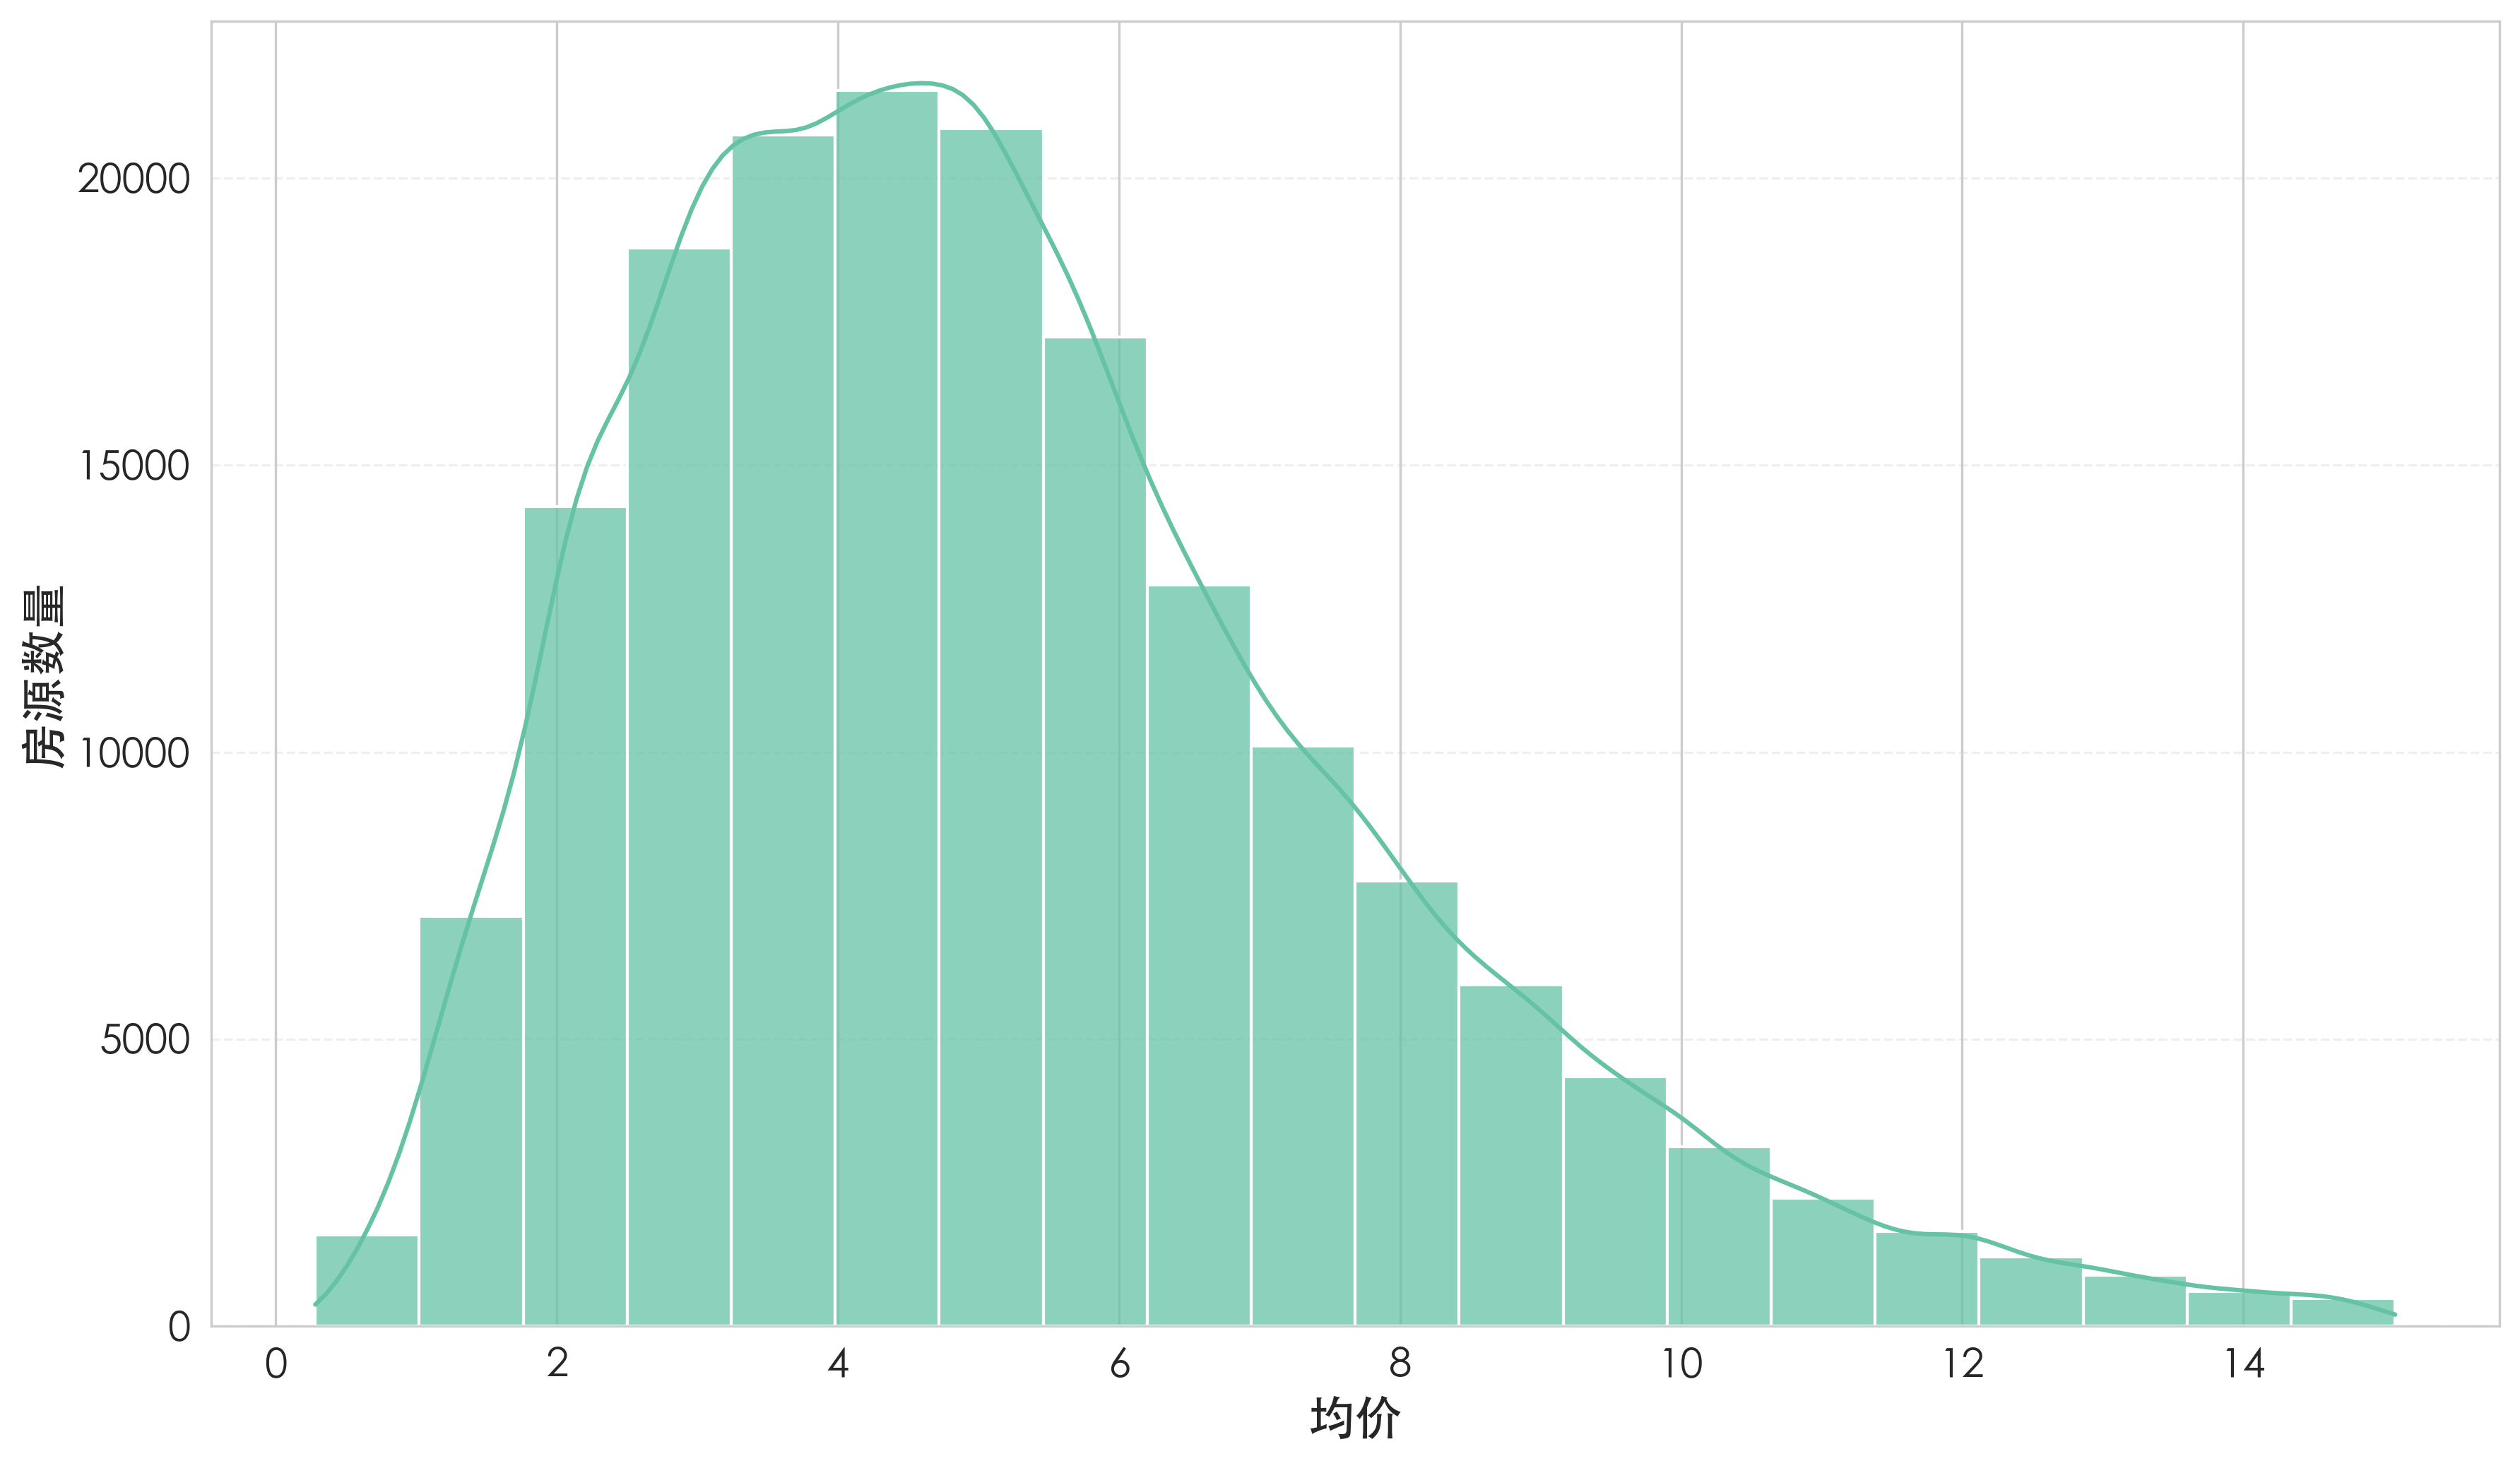
\includegraphics[width=1\textwidth]{hist_均价.png}
  \caption{均价分布直方图}
  \label{fig:fig1}
\end{figure}

\subsubsection{房源基本属性自变量分析}

房源基本属性自变量主要涵盖居室数、厅堂数、卫生间数、房屋总面积、装修类型与楼层位置，本节针对上
述特征变量开展单因子房价差异分析。居室数、厅堂数与二手房均价的分组箱线图分别如图 \ref {fig:jushi} 和
图 \ref {fig:tingtang} 所示。从居室结构来看，上海二手房房源主要集中在两室、三室户型。
其中两室户型均价水平最低；一室户型受户型稀缺性及小户型单价偏高特征影响，均价反而高于两室户型；
三室、四室、五室及以上户型的房源均价则呈现逐级上升趋势。与之相对，厅堂布局主要以一厅、二厅为主，
两类房源的单位均价差异较小；而三厅及以上大格局房源均价出现明显抬升，但此类房源存量稀缺，样本占比仅为 3\%。
卫生间数量同样表现出相近的价格分异特征，房源以 0–1 卫配置为主，多卫生间户型的二手房均价显著更高，
具体分布特征如图 \ref {fig:wsj} 所示。居室数、厅堂数、卫生间数量三者与房屋总面积存在高度相关性。
绘制按均价分组堆叠的房屋总面积分布直方图，结果如图 \ref {fig:zmj1} 所示：房屋总面积整体呈右偏分布，
房源面积主要集中在 50-150㎡区间，面积超过 100㎡后房源频数明显回落；同时随着建筑面积增大，
均价 3 万元 /㎡以下的刚需房源占比逐步下降。对房屋总面积进行区间分组并绘制均价箱线图，
如图 \ref {fig:zmj2} 所示，其价格变化规律与居室数等变量基本一致。70-100㎡区间房源均价最低，
100-150㎡改善型房源、150㎡及以上大户型房源均价依次攀升，体现出居住空间尺度对二手房价格具有
显著的正向拉动作用。从装修类型（图\ref {fig:zx}）的箱线图来看，从毛坯、简装、精装修、豪华装修呈现房价逐级上升的
趋势，从样本结构看，市场流通房源以精装修为主，占据绝对市场份额。
在楼层位置方面，低层、中层与高层房源的均价并未表现出显著分异特征，不同楼层间价格差异不明显，因此本文不再对楼层位置作进一步展开分析。


 \begin{figure}[htbp]
  \centering
  \begin{minipage}[t]{0.45\textwidth}
    \centering
    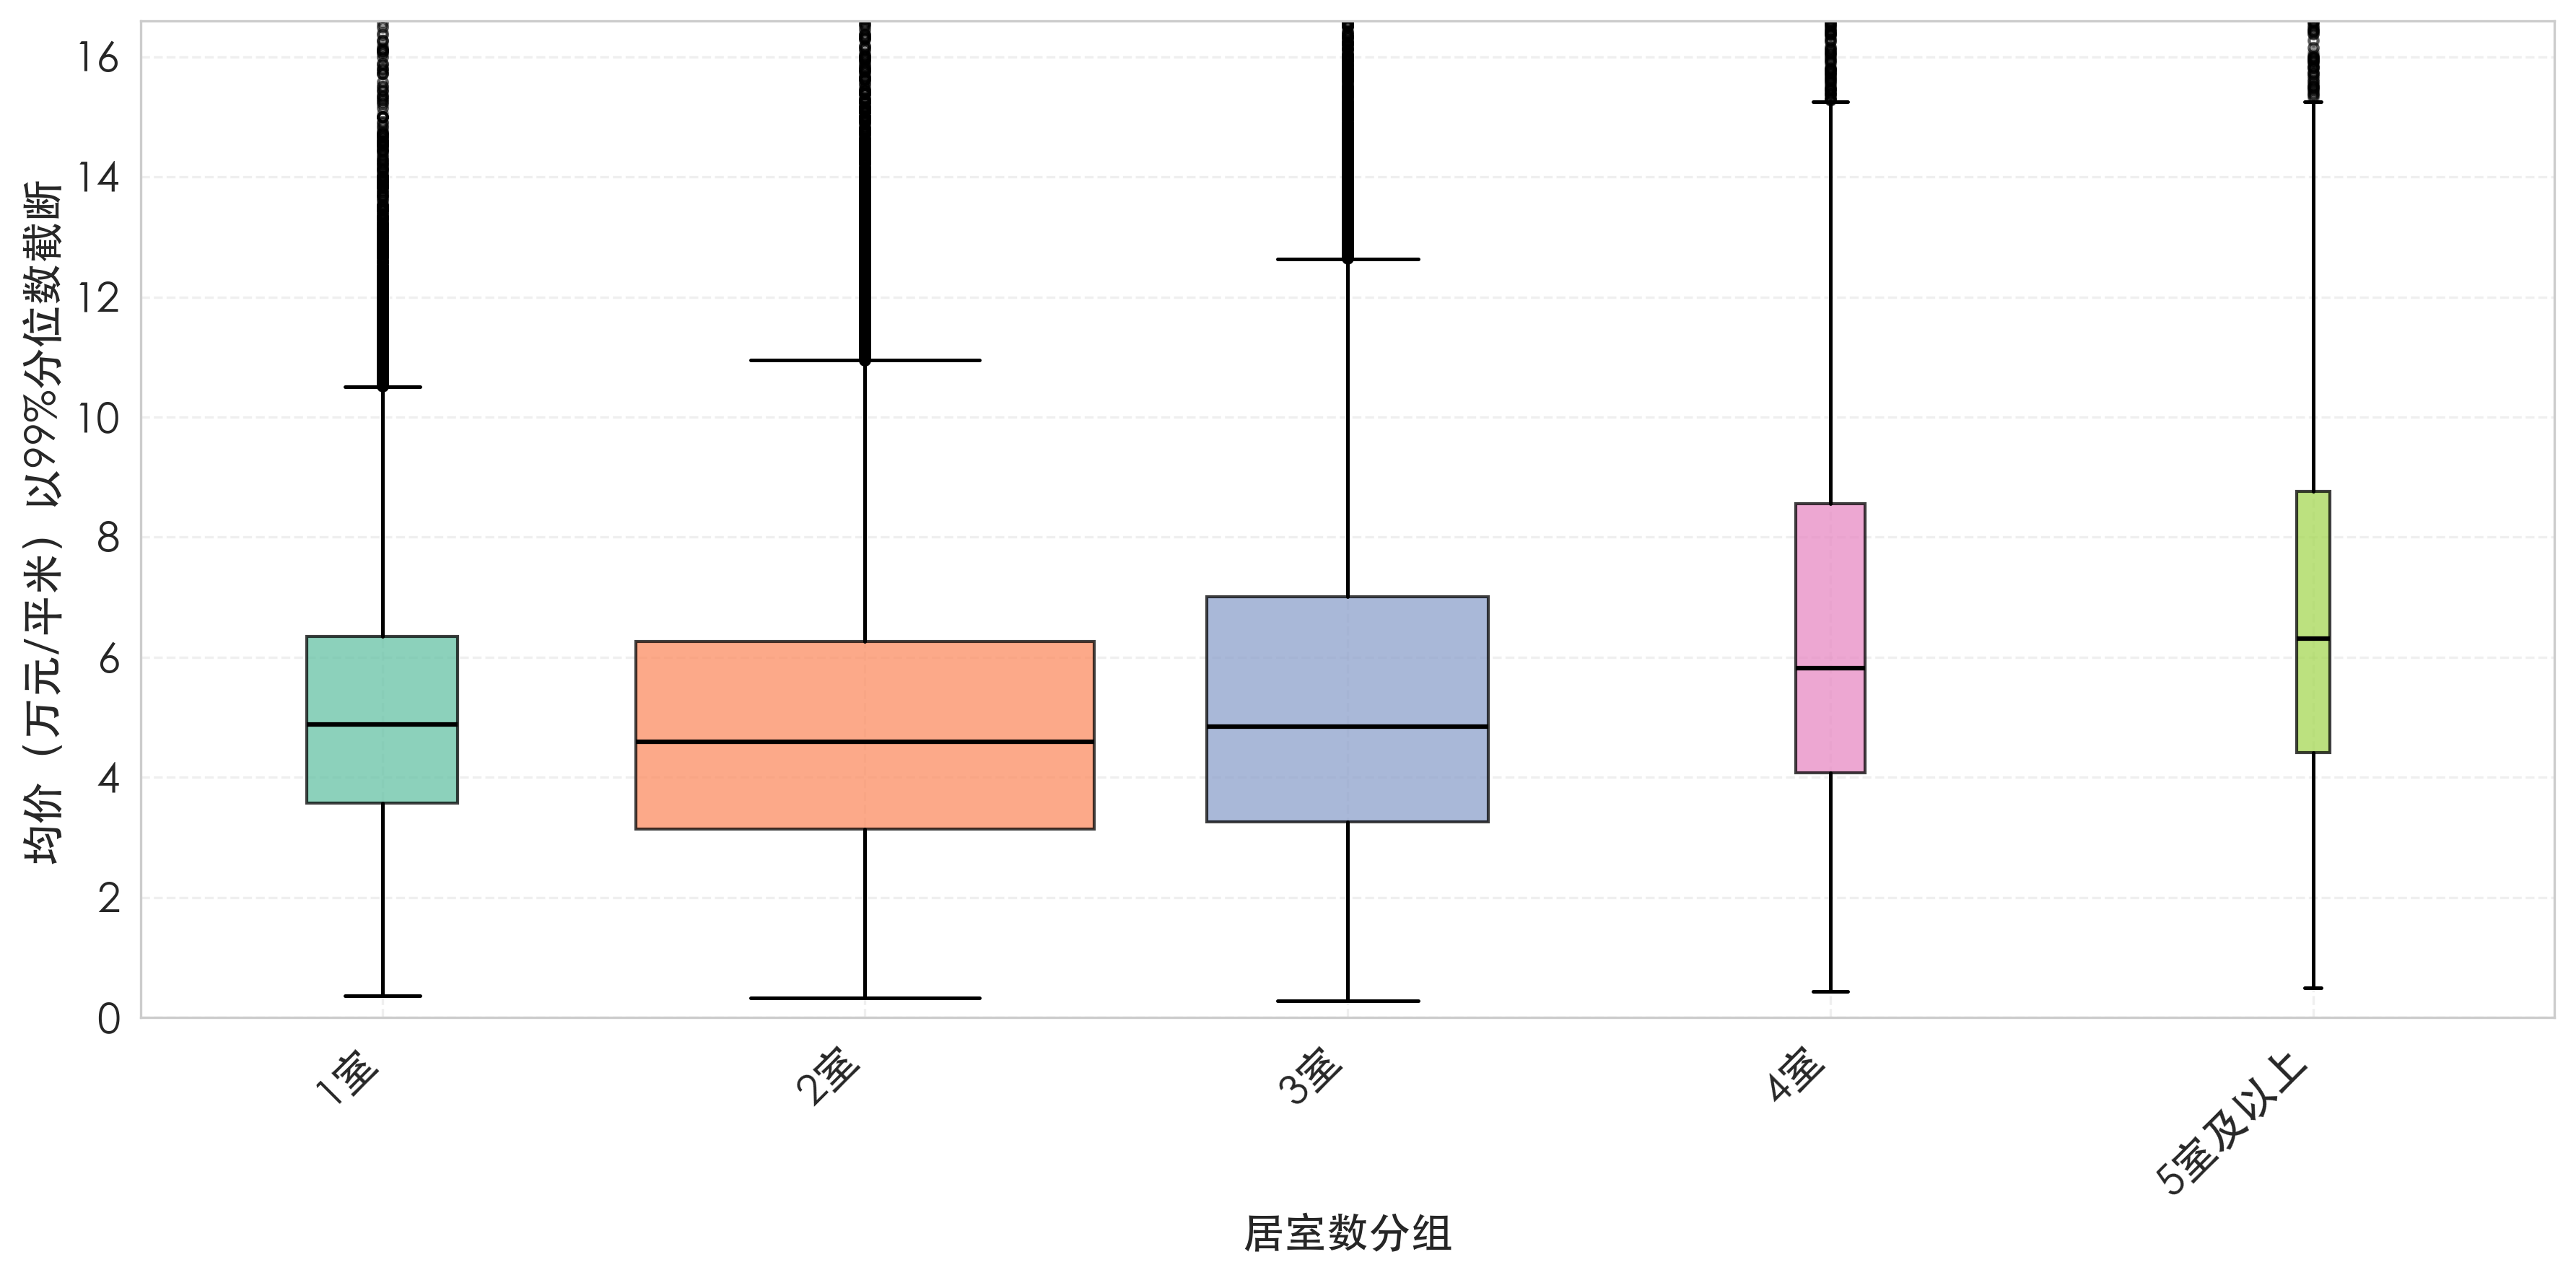
\includegraphics[width=\linewidth]{boxplot_居室数分组.png}
    \caption{居室数分组-均价箱线图} % 图标题
    \label{fig:jushi} 
  \end{minipage}
  \hfill
  \begin{minipage}[t]{0.45\textwidth}
    \centering
    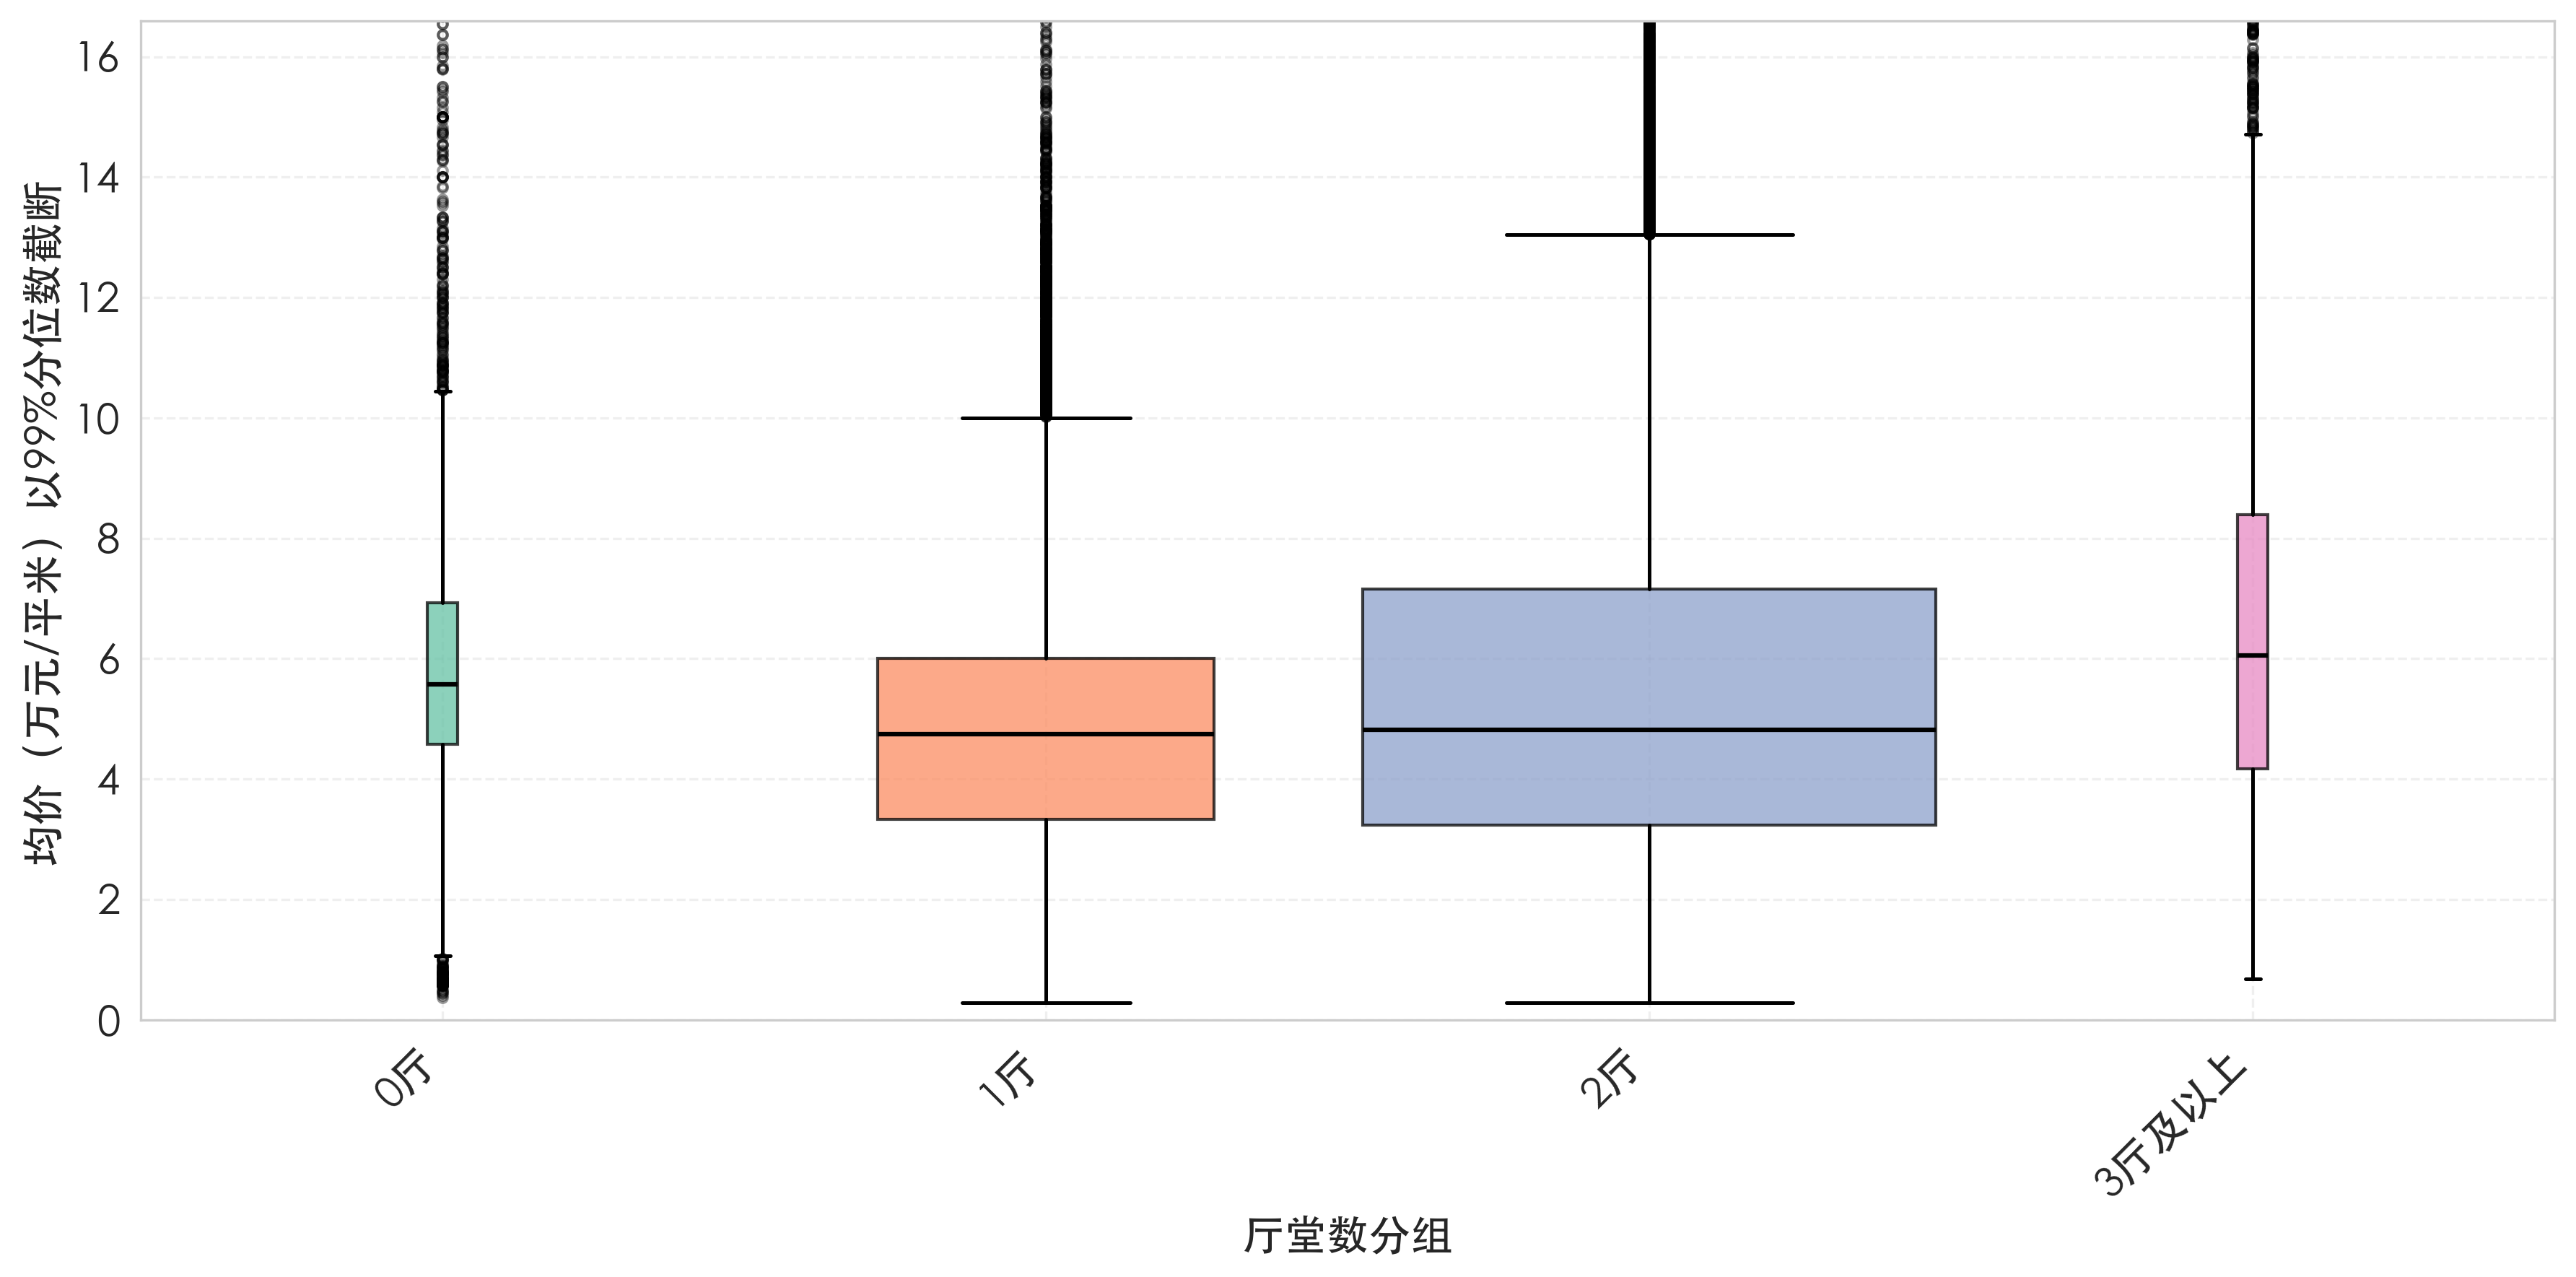
\includegraphics[width=\linewidth]{boxplot_厅堂数分组.png}
    \caption{厅堂数分组-均价箱线图} % 图标题
    \label{fig:tingtang} 
  \end{minipage}
\end{figure}


 \begin{figure}[htbp]
  \centering
  \begin{minipage}[t]{0.45\textwidth}
    \centering
    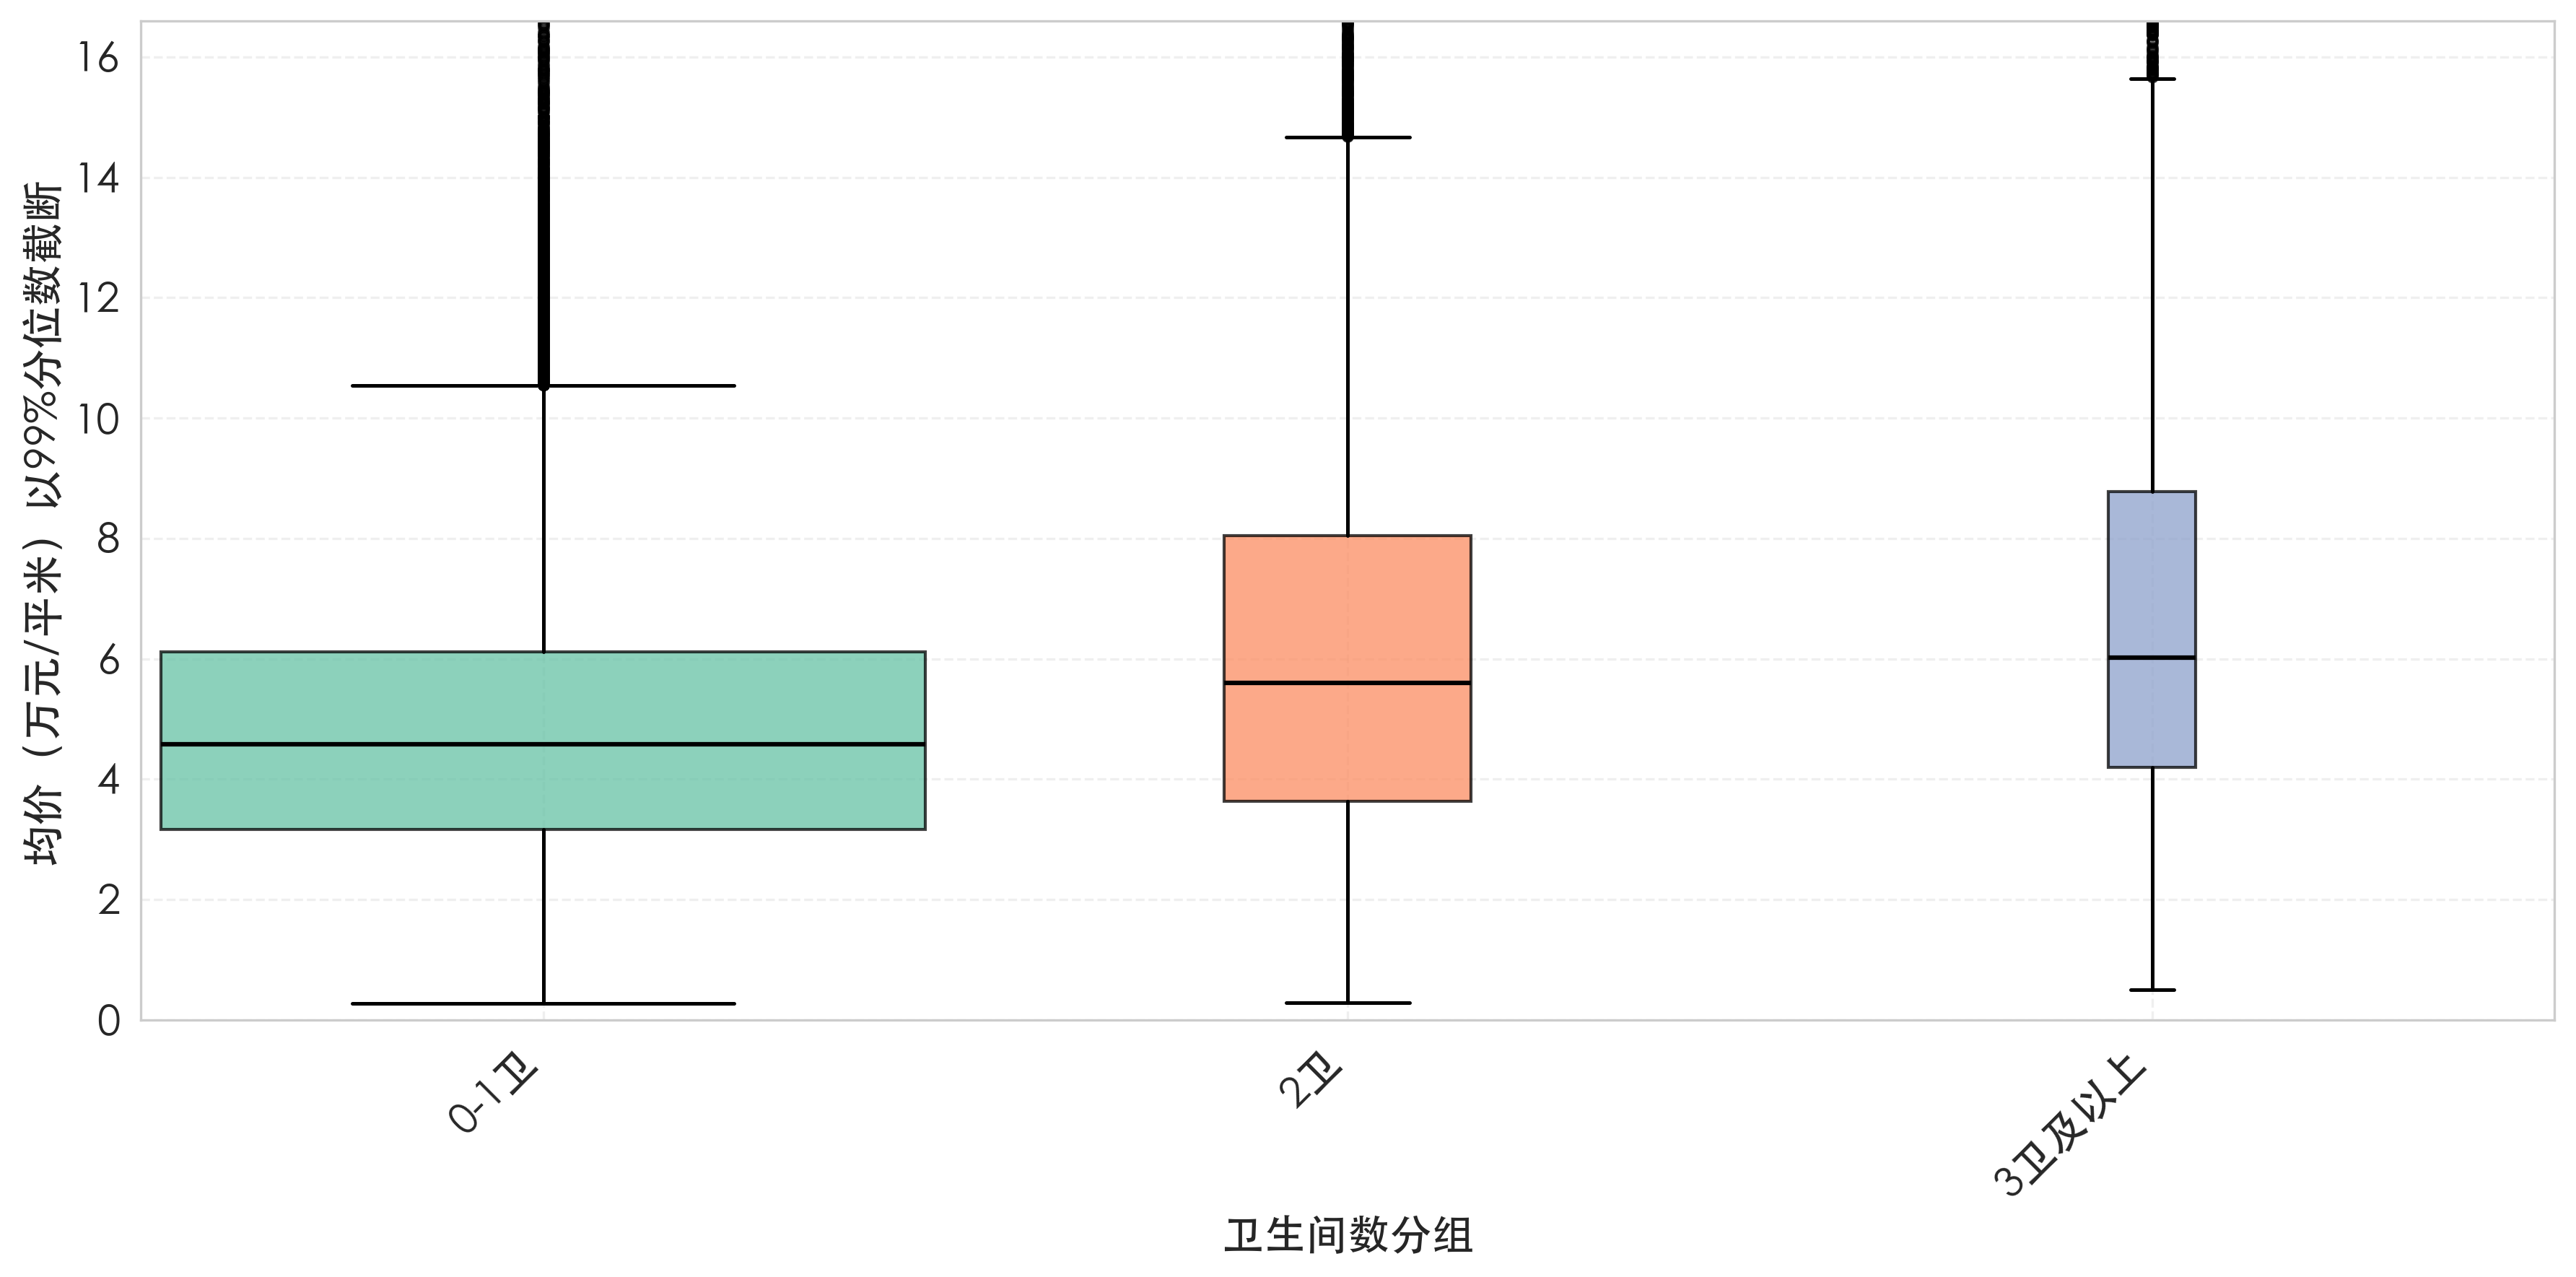
\includegraphics[width=\linewidth]{boxplot_卫生间数分组.png}
    \caption{卫生间数分组-均价箱线图} % 图标题
    \label{fig:wsj} 
  \end{minipage}
  \hfill
  \begin{minipage}[t]{0.45\textwidth}
    \centering
    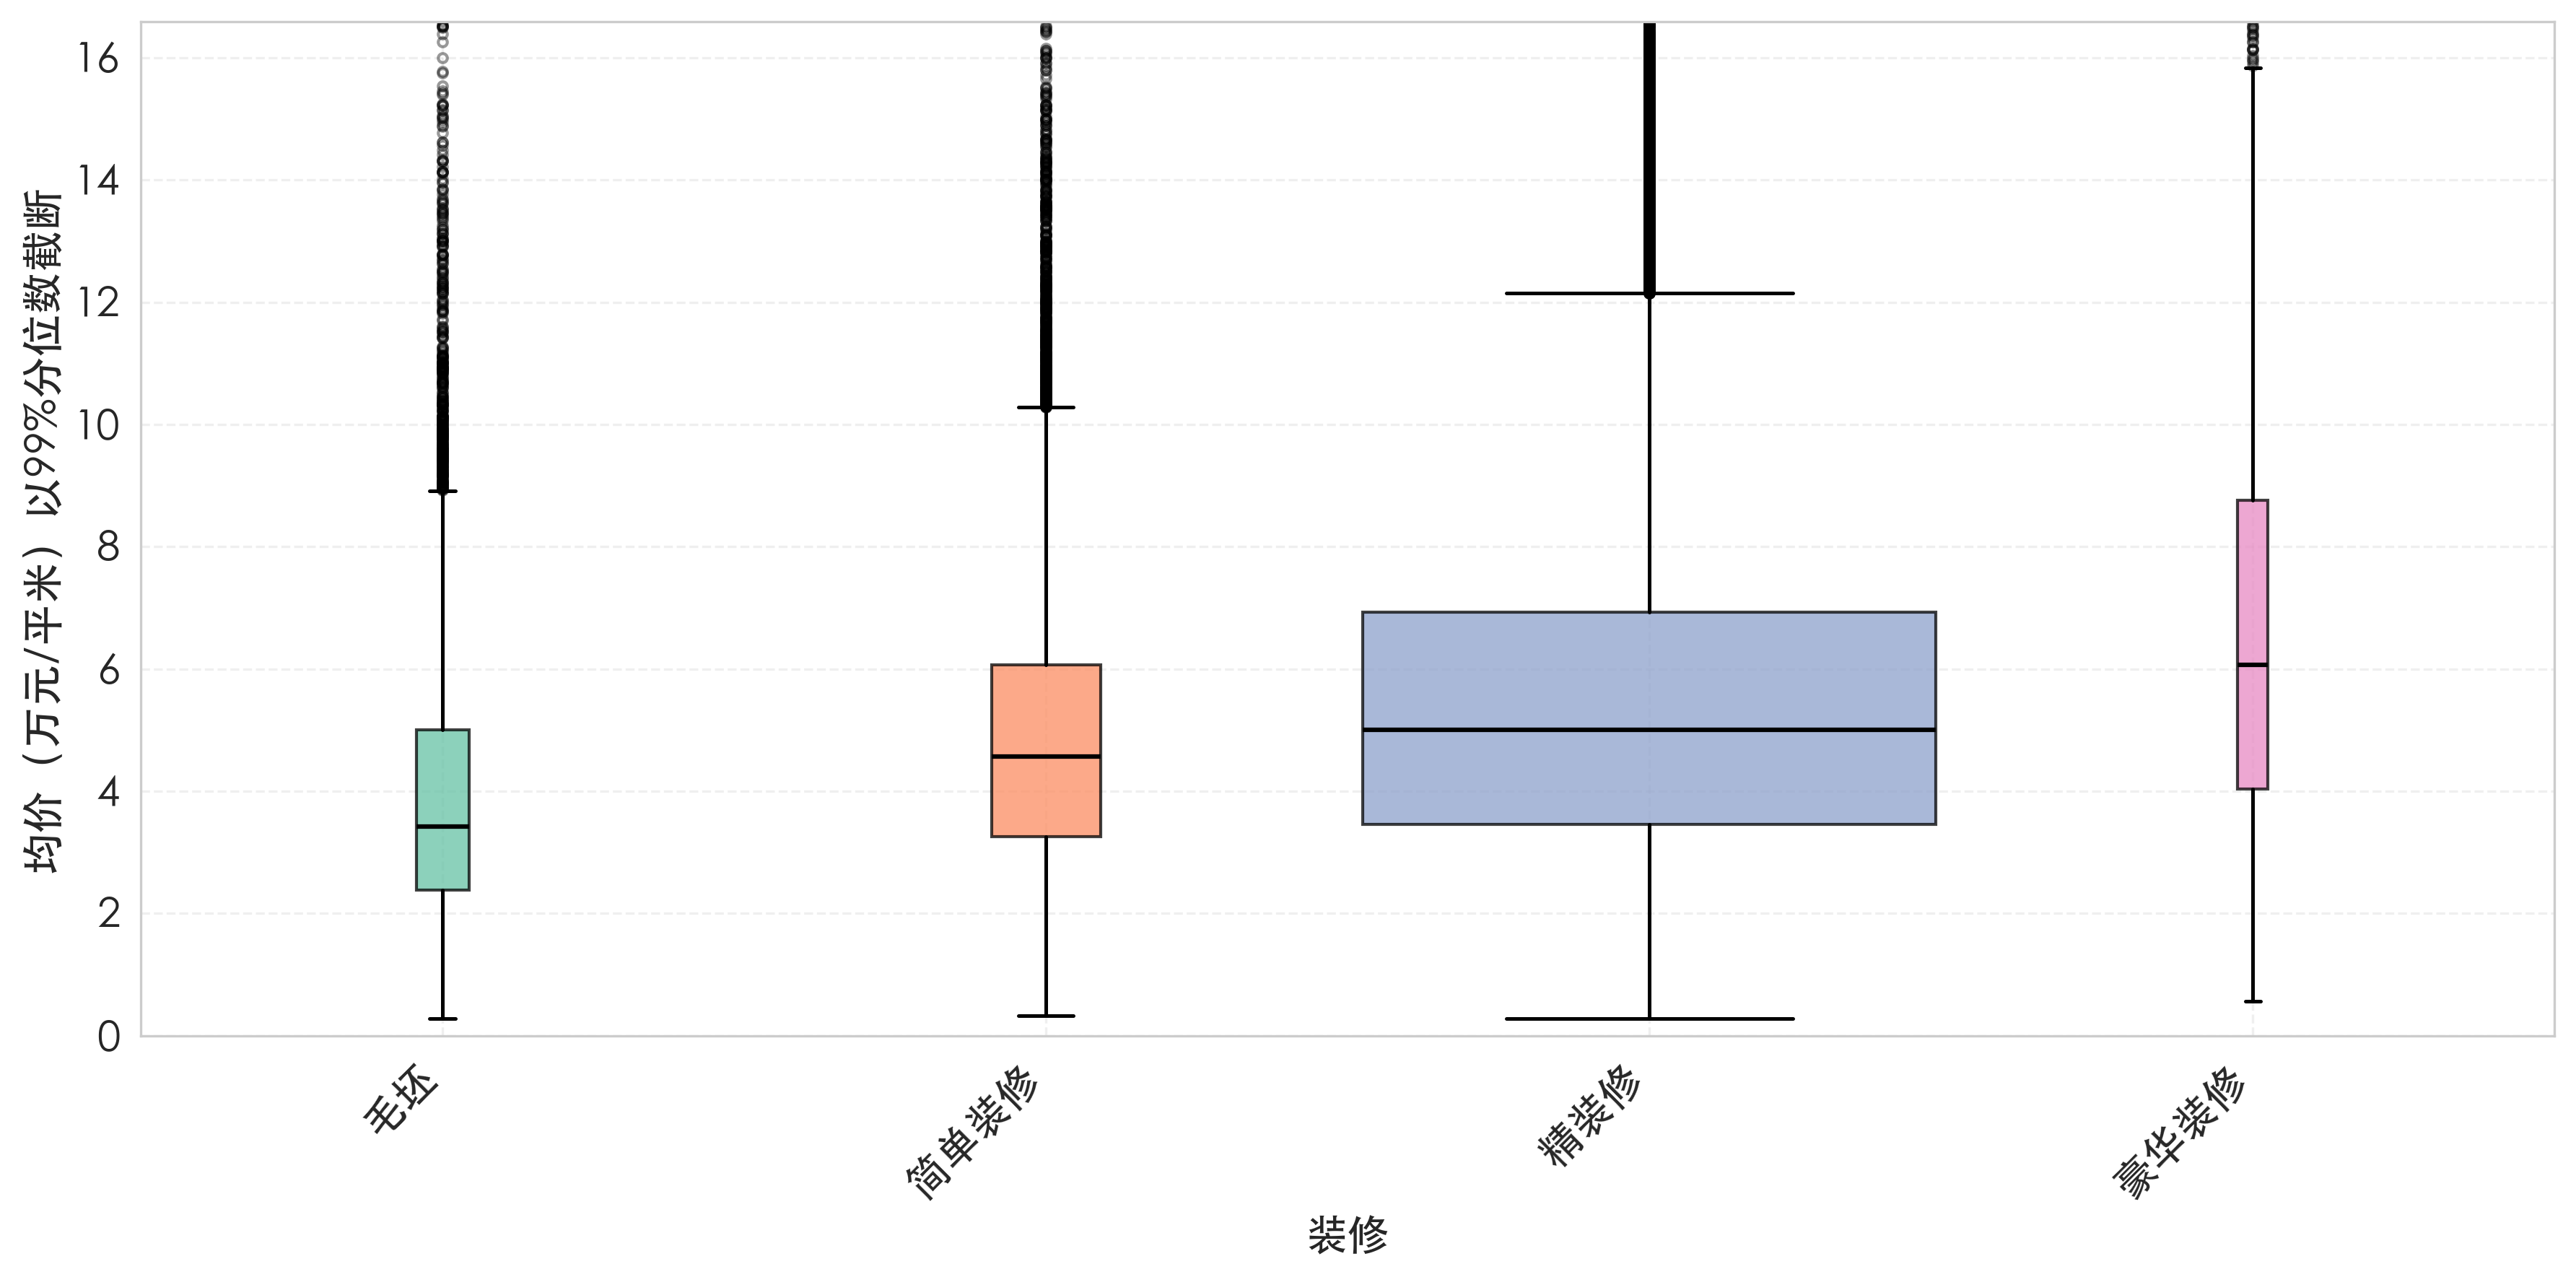
\includegraphics[width=\linewidth]{boxplot_装修.png}
    \caption{装修类型-均价箱线图} 
    \label{fig:zx} 
  \end{minipage}
\end{figure}

 \begin{figure}[htbp]
  \centering
  \begin{minipage}[t]{0.45\textwidth}
    \centering
    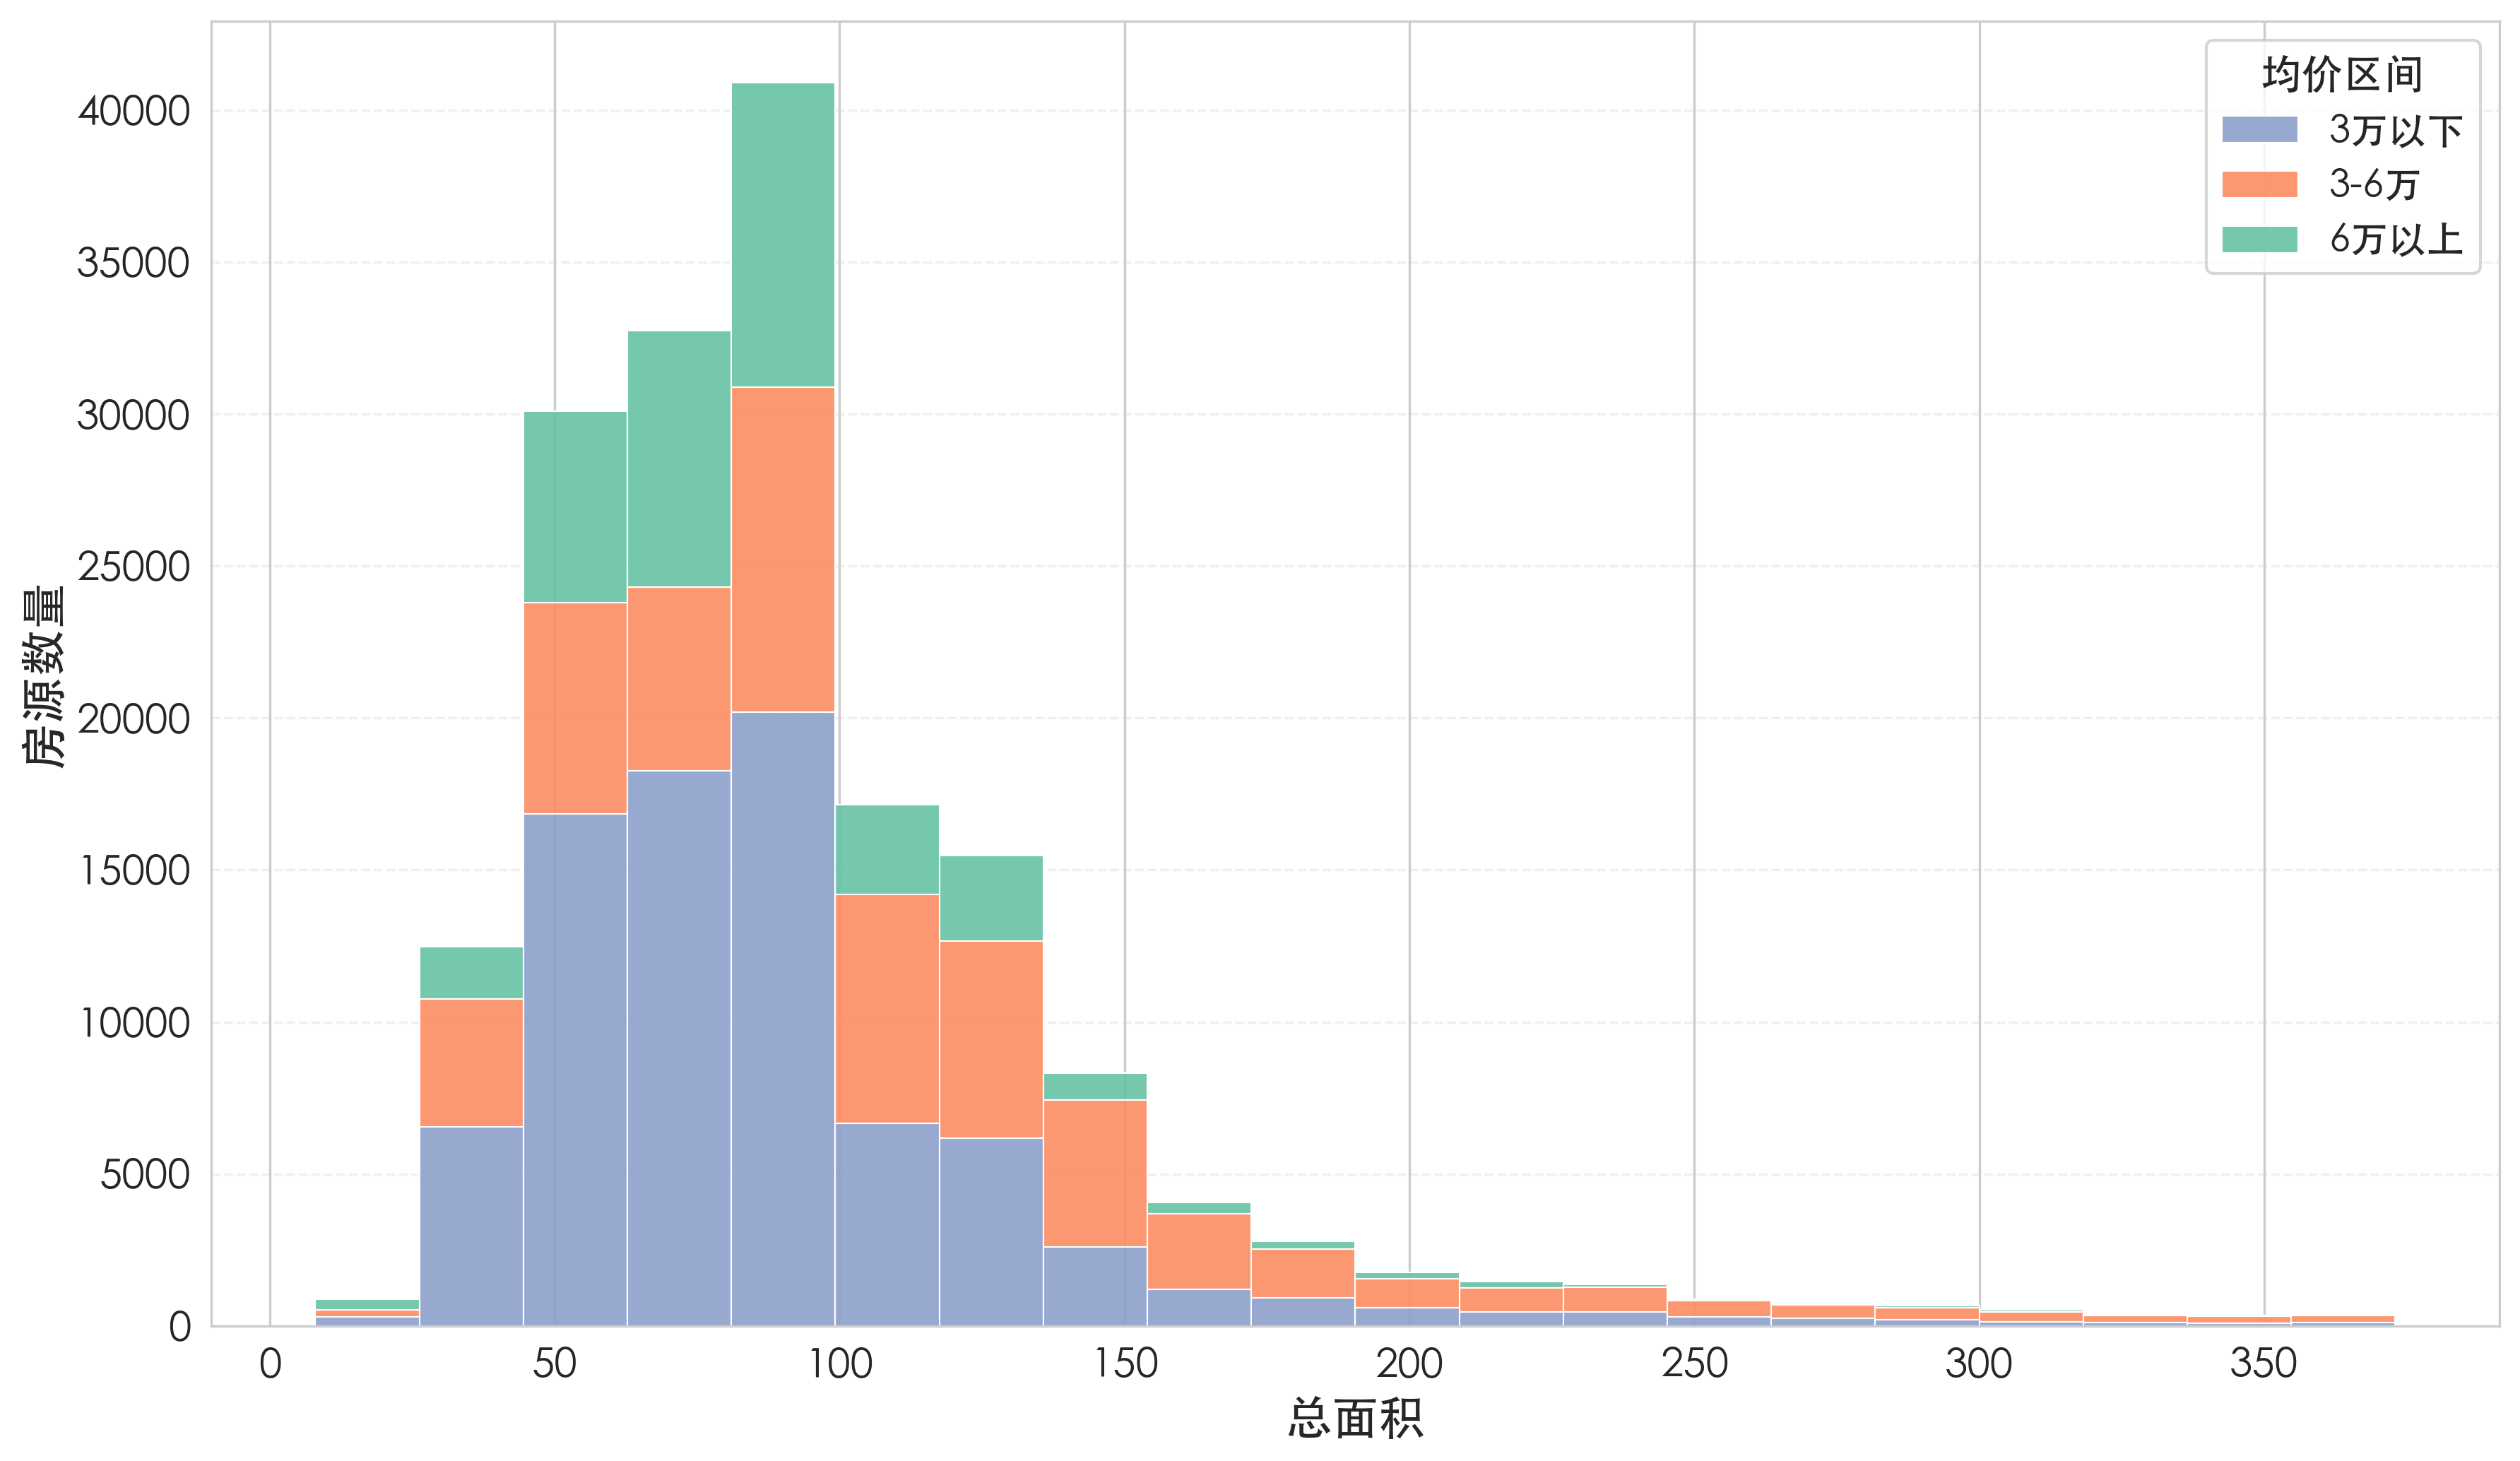
\includegraphics[width=\linewidth]{hist_总面积_均价分组.png}
    \caption{总面积-均价分组直方图} % 图标题
    \label{fig:zmj1} 
  \end{minipage}
  \hfill
  \begin{minipage}[t]{0.45\textwidth}
    \centering
    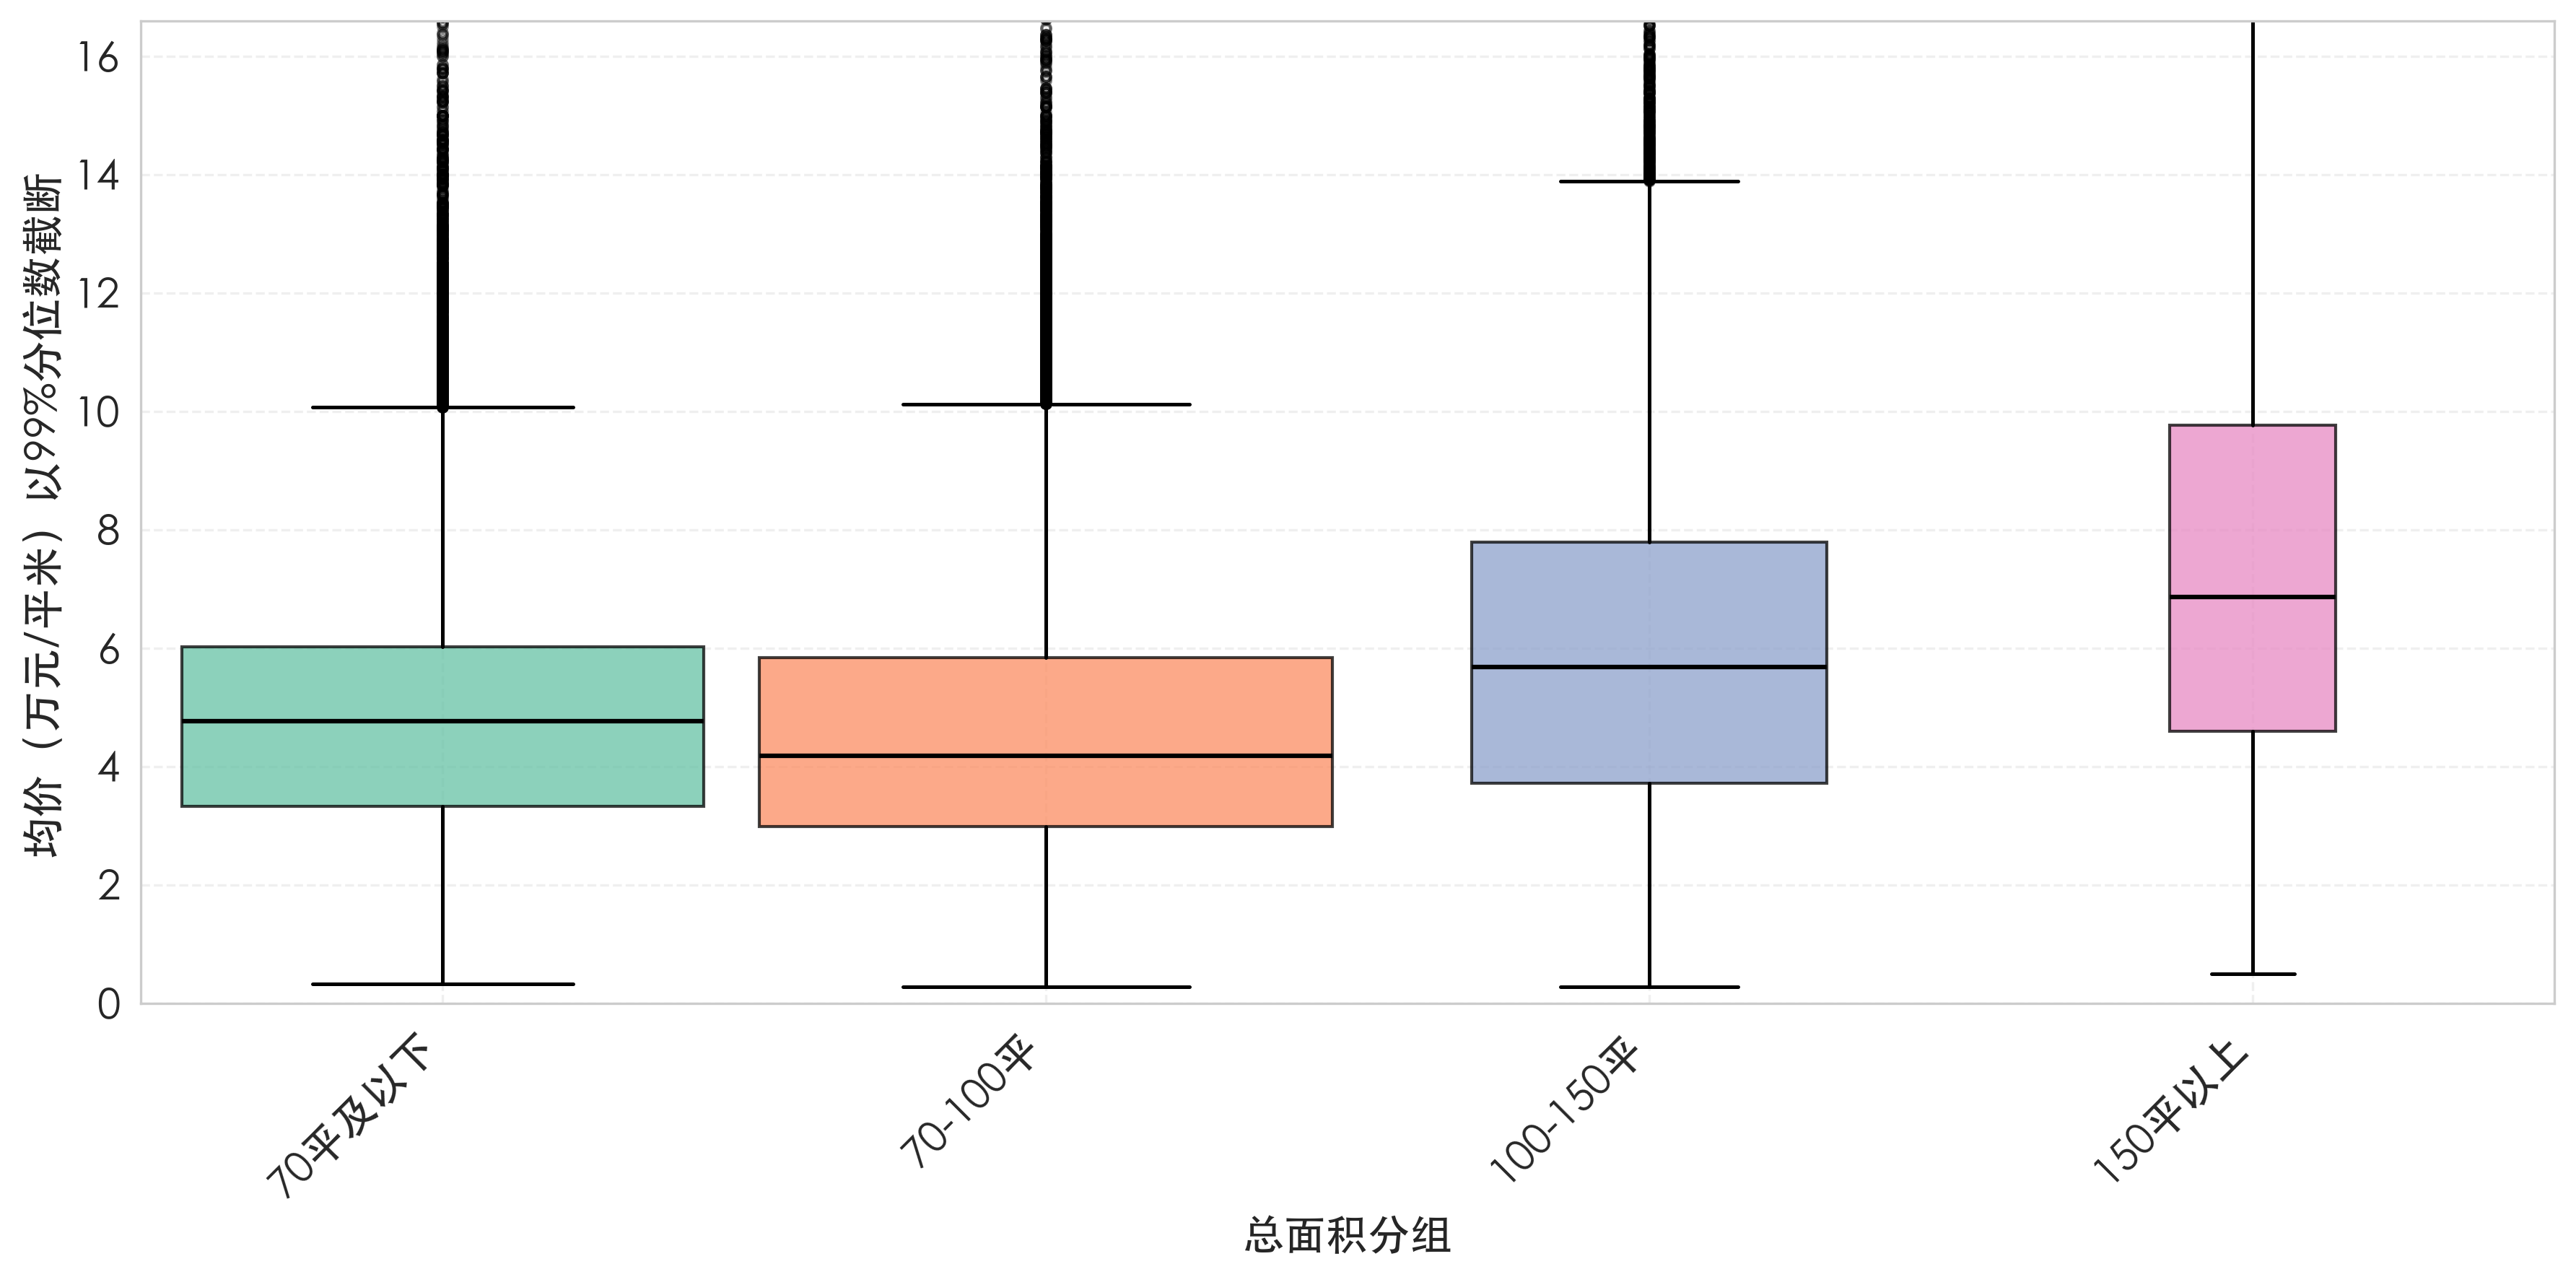
\includegraphics[width=\linewidth]{boxplot_总面积分组.png}
    \caption{总面积分组-均价箱线图} 
    \label{fig:zmj2} 
  \end{minipage}
\end{figure}


\subsubsection{字符型自变量分析：户型、装修情况、房屋朝向等分布特征}



\subsection{相关性分析} 

\subsubsection{房价与建筑属性、小区属性等的相关性分析} 

\subsubsection{变量相关性热力图与多重共线性判断}

\subsection{基于经纬度的空间分布分析}

\subsubsection{上海市二手房房价整体空间分布格局}

\subsubsection{各行政区 / 板块房价的空间差异与聚类特征}

\subsubsection{核心 POI 对房价的空间影响分析}

\section{实证分析}

\subsection{关键影响变量识别-LASSO 回归模型构建与最优正则化参数选择} 

\subsection{用GLM构建基准模型} 

\subsection{分析基准模型的残差，进行空间效应检验}

\subsection{相同的解释变量构建空间模型}

\subsection{两个模型的解读和拟合效果对比}

\section{结论与总结}

\end{document} 
